% Chapter 3 -- Methodology (\input by main.tex): detection pipeline + object completion
% (completion half merged in below, formerly sec_6_completion_method.tex).
%
% Honesty-phrasing rules applied (personal_agenda P1):
%   - production classifier is the FROM-SCRATCH Stage B checkpoint
%     (stage_b_scratch_best.pth, Finding #31); synthetic Stage A pretraining
%     was DROPPED from the final pipeline and is kept only as Ch-4 ablation
%     material (#25/#30). We do NOT present two-stage training as a contribution.
%   - measured vs inferred evidence tiers marked in prose; timing numbers are
%     measured (timing_seq08_full_n4068.json), cited as such.
%   - every number traceable to a finding / output artifact.
%   - "the classifier's job is precision" claim deferred to the Ch-4 ablation.
%
\chapter{Proposed Methodology}
\label{ch:pipeline}

This chapter presents the proposed method: a modular detection and completion framework
for automotive LiDAR. Section~\ref{sec:meth-architecture} gives the overall architecture;
the sections that follow describe each stage in the order a scan flows through it, in its
configured, instantiated form. The general operators each stage is built from are defined
in Chapter~\ref{ch:background}; this chapter states how each is set up and connected here,
and the end-to-end evaluation is Chapter~\ref{ch:evaluation}.

\section{System Architecture}
\label{sec:meth-architecture}

The framework is a single system that turns a raw LiDAR scan into completed,
box-estimated cars. It is organised as two stages in sequence, each the subject of one
section below. The detection stage (Section~\ref{sec:meth-detection}) segments and
classifies car clusters from the raw scan, emitting an oriented bounding box and a stable
track identity per car. The completion stage (Section~\ref{ch:completion-method})
reconstructs each detected car's full surface from the one-sided partial a single frame
observes. Figure~\ref{fig:architecture} shows this two-stage organisation, and
Figure~\ref{fig:pipeline} details the detection chain that produces every input the
completion stage consumes.

The design is deliberately modular and classical: classical geometry does the work
geometry solves well, and small learned models are used only where discrimination
needs them, so every stage is separately inspectable and its cost separately
measurable. This architecture is what lets the evaluation
(Chapter~\ref{ch:evaluation}) attribute the recall limit to a single stage rather than
to an opaque network.

\begin{figure}[H]
  \centering
  \begin{tikzpicture}[
      font=\small,
      >=Stealth,
      stage/.style={draw, rounded corners, align=center, thick,
        minimum width=58mm, minimum height=16mm, fill=blue!5},
      ltag/.style={draw, rounded corners, align=center, thick,
        font=\footnotesize, fill=orange!12, minimum width=22mm, minimum height=10mm},
      io/.style={draw, ellipse, align=center, fill=black!5,
        minimum width=44mm, minimum height=10mm},
      arr/.style={-{Stealth[length=2.2mm]}, thick},
      legsq/.style={draw, rounded corners, minimum width=5mm, minimum height=3.5mm},
    ]
    \node[io] (raw) {Raw LiDAR scan};
    \node[stage, below=9mm of raw] (det)
      {\textbf{Detection}\\[1pt]
       {\footnotesize preprocess $\cdot$ ground removal $\cdot$ clustering}\\
       {\footnotesize geometric filter $\cdot$ classifier $\cdot$ tracking}};
    \node[ltag, right=10mm of det] (detL) {car / not-car\\classifier};
    \node[io, below=9mm of det] (mid) {Car detections\\{\footnotesize oriented boxes + track ids}};
    \node[stage, below=9mm of mid] (comp)
      {\textbf{Completion}\\[1pt]
       {\footnotesize L-shape gate $\cdot$ canonical normalisation}\\
       {\footnotesize $\cdot$ length geometry $\cdot$ re-projection}};
    \node[ltag, right=10mm of comp] (compL) {PCN\\network};
    \node[io, below=9mm of comp] (out) {Completed cars\\{\footnotesize dense surface + box}};

    \draw[arr] (raw) -- (det);
    \draw[arr] (det) -- (mid);
    \draw[arr] (mid) -- (comp);
    \draw[arr] (comp) -- (out);
    \draw[densely dashed, black!55] (det.east) -- (detL.west);
    \draw[densely dashed, black!55] (comp.east) -- (compL.west);

    \node[legsq, fill=blue!5, below=8mm of out, xshift=-30mm] (lc) {};
    \node[right=1.5mm of lc, font=\scriptsize] (lct) {classical (training-free)};
    \node[legsq, fill=orange!12, right=8mm of lct] (ll) {};
    \node[right=1.5mm of ll, font=\scriptsize] {learned model};
  \end{tikzpicture}
  \caption[System architecture]{The two-stage system architecture: a detection stage
    (Section~\ref{sec:meth-detection}) feeds a completion stage
    (Section~\ref{ch:completion-method}). Both are built mostly from classical geometry with
    a single small learned model each (shaded): the car/not-car classifier and the PCN
    network. Figures~\ref{fig:pipeline} and~\ref{fig:completion-pipeline} expand the two
    stages.}
  \label{fig:architecture}
\end{figure}

\section{Detection Pipeline}
\label{sec:meth-detection}

This section describes the car detection pipeline that produces every detection
evaluated in Chapter~\ref{ch:evaluation} and every cluster completed in
Section~\ref{ch:completion-method}. The
design is deliberately modular and classical: a chain of independent stages,
each with a small number of interpretable parameters, rather than an end-to-end
learned detector. This choice trades peak accuracy for interpretability,
reproducibility, and zero additional manual annotation: the classifier is trained on
labels mined automatically from existing semantic annotations
(Section~\ref{sec:pipeline-classifier}). It is also what lets Section~\ref{sec:recall-analysis}
root cause the recall shortfall to a single stage rather than to an opaque
network.

The pipeline takes one raw LiDAR scan and emits a set of car detections, each an
oriented bounding box with a stable track identity across frames. Every stage
parameter lives in a single frozen configuration, fixed before the write up began; the frozen
values are collected in Table~\ref{tab:pipeline-config}. Figure~\ref{fig:pipeline}
gives the full chain.

\subsection{Overview of the Modular Detection Pipeline}
\label{sec:pipeline-overview}

\begin{figure}[H]
  \centering
  \begin{tikzpicture}[
      font=\small,
      node distance=6mm,
      stage/.style={
        draw, rounded corners, align=center,
        minimum width=34mm, minimum height=11mm,
        fill=blue!5, thick},
      learned/.style={stage, fill=orange!12},
      io/.style={draw, ellipse, align=center, fill=black!5,
        minimum width=28mm, minimum height=9mm},
      ms/.style={font=\footnotesize\itshape, text=black!60},
      arr/.style={-{Stealth[length=2.2mm]}, thick},
      grp/.style={draw=black!45, dashed, rounded corners, inner sep=3mm},
      grplab/.style={font=\footnotesize\bfseries, text=black!65},
      legsq/.style={draw, rounded corners, minimum width=5mm, minimum height=3.5mm},
    ]
    \node[io] (raw) {Raw LiDAR scan};
    \node[stage, below=of raw] (pre) {Preprocess\\{\footnotesize $z$-filter $\to$ voxel $\to$ denoise}};
    \node[stage, below=of pre] (ground) {Ground removal\\{\footnotesize RANSAC plane}};
    \node[stage, below=of ground] (cluster) {Clustering\\{\footnotesize HDBSCAN @ \SI{0.10}{\meter}}};
    \node[stage, below=12mm of cluster] (geo) {Geometric filter\\{\footnotesize OBB gates}};
    \node[learned, below=of geo] (clf) {Classification\\{\footnotesize PointNet, car/not-car}};
    \node[stage, below=of clf] (track) {Tracking\\{\footnotesize centroid + track vote}};
    \node[io, below=of track] (out) {Car detections\\{\footnotesize boxes + track ids}};

    \draw[arr] (raw) -- (pre);
    \draw[arr] (pre) -- (ground);
    \draw[arr] (ground) -- (cluster);
    \draw[arr] (cluster) -- (geo);
    \draw[arr] (geo) -- (clf);
    \draw[arr] (clf) -- (track);
    \draw[arr] (track) -- (out);

    % dashed phase blocks (segmentation: points -> clusters; detection: clusters -> cars)
    \begin{scope}[on background layer]
      \node[grp, fit=(pre)(ground)(cluster)] (segbox) {};
      \node[grp, fit=(geo)(clf)(track)] (detbox) {};
    \end{scope}
    \node[grplab, rotate=90] at ([xshift=-4mm]segbox.west) {Segmentation};
    \node[grplab, rotate=90] at ([xshift=-4mm]detbox.west) {Detection};

    % per-stage output in one column, anchored to the phase-block right edge (uniform gap)
    \node[ms, anchor=west] at ([xshift=6mm]segbox.east|-pre)     {$\to$ cleaned points};
    \node[ms, anchor=west] at ([xshift=6mm]segbox.east|-ground)  {$\to$ non-ground points};
    \node[ms, anchor=west] at ([xshift=6mm]segbox.east|-cluster) {$\to$ object clusters};
    \node[ms, anchor=west] at ([xshift=6mm]detbox.east|-geo)     {$\to$ car candidates};
    \node[ms, anchor=west] at ([xshift=6mm]detbox.east|-clf)     {$\to$ car clusters};
    \node[ms, anchor=west] at ([xshift=6mm]detbox.east|-track)   {$\to$ tracked cars};

    \node[legsq, fill=blue!5] (lc) at ([yshift=-10mm]out.south west) {};
    \node[right=1.5mm of lc, font=\scriptsize] (lct) {classical (training-free)};
    \node[legsq, fill=orange!12, right=8mm of lct] (ll) {};
    \node[right=1.5mm of ll, font=\scriptsize] {learned};
  \end{tikzpicture}
  \caption[Detection pipeline]{The detection pipeline, grouped into two phases (dashed): a
    segmentation phase that turns a raw scan into clusters (preprocess, ground removal,
    clustering) and a detection phase that turns clusters into tracked car boxes
    (geometric filter, classification, tracking), with each stage's output shown at right.
    Learned stages are shaded; all others are classical.}
  \label{fig:pipeline}
\end{figure}

The system is offline by design: the tracker and the track-level filter
use the whole sequence, and real-time operation is out of scope. The pipeline runs well
below sensor rate, and the per stage runtime budget, which stages dominate, and where
the learned and classical costs fall, is measured and reported in the runtime section
of Chapter~\ref{ch:evaluation} rather than claimed here.

\subsection{Preprocessing: Filtering, Downsampling, and Denoising}
\label{sec:pipeline-preprocess}

\noindent \textbf{Input:} raw LiDAR scan \quad \textbar \quad \textbf{Output:} cleaned point cloud (height-filtered, voxel-downsampled, denoised) \vspace{0.5em}

Each raw scan passes through three cleaning steps
before any object reasoning:

\begin{enumerate}
  \item Ground height $z$-filter. Points below
    $z = \SI{-2.0}{\meter}$ in the sensor frame are dropped. This removes the bulk
    of the road surface and any sub-ground noise cheaply, before the more
    expensive steps see them.
  \item Voxel downsampling at \SI{0.05}{\meter}. Points are collapsed to
    one representative per \SI{5}{\centi\meter} voxel, which both regularises the
    range dependent density of LiDAR and cuts the point count by roughly an order
    of magnitude.
  \item Statistical outlier removal. Points whose mean distance to their
    \num{20} nearest neighbours exceeds \num{2.0} standard deviations of the
    local distribution are discarded, removing isolated speckle.
\end{enumerate}

The order of the last two steps is behaviour changing. In the frozen configuration,
downsampling runs before
denoising, so the statistical outlier test operates on roughly ten times fewer
points, and on a regularised point set, which changes which points survive.
This ordering was adopted as part of the pipeline optimisation primarily
because it improves detection (Chapter~\ref{ch:evaluation}). It is behaviour changing, so
we flag it here rather than presenting the two orderings as equivalent.

\subsection{Ground Plane Removal by RANSAC}
\label{sec:pipeline-ground}

\noindent \textbf{Input:} cleaned point cloud \quad \textbar \quad \textbf{Output:} non-ground (object) points $+$ fitted ground plane \vspace{0.5em}

The dominant remaining structure after preprocessing is the ground plane, which
must be removed before clustering or it bridges every object into one component.
We fit a single plane with RANSAC: over \num{300} iterations, three points are
sampled, their plane computed, and inliers counted within
\SI{0.2}{\meter}; the best supported plane is kept. The plane is
accepted only if its normal is near vertical (the $z$-component of the
unit normal must exceed \num{0.5}), so a spuriously fitted vertical surface (a
wall, the side of a truck) cannot be mistaken for ground. If the check fails, no
points are removed and the whole cloud is passed on as objects; this fail safe is
rare but prevents a bad plane fit from deleting real cars.

A single global plane is a deliberate simplification: it assumes the local ground
is approximately planar, which holds on the flat urban sequences used here but
would degrade on strong slopes. A grid-based ground model (Patchwork++-style) is
listed as future work, not a limitation we claim to have solved. The iteration
count was reduced from \num{1000} to \num{300} as part of the runtime optimisation after
confirming the plane fit converges well before \num{1000} iterations on this
data. The fit uses a fixed random seed (\num{42}), so ground
removal, and therefore the whole pipeline, is deterministic across runs.

\subsection{Object Candidate Clustering with HDBSCAN}
\label{sec:pipeline-cluster}

\noindent \textbf{Input:} non-ground points \quad \textbar \quad \textbf{Output:} object clusters \vspace{0.5em}

Non-ground points are grouped into object candidates with HDBSCAN
(Section~\ref{sec:th-clustering} gives the general mutual reachability construction), here
configured with a minimum cluster size of \num{10} and a minimum samples value of \num{5}
(the neighbour count $m$ that sets the core distance). HDBSCAN is chosen over a fixed radius method
because LiDAR density falls off with range: a single Euclidean radius that merges
nothing at \SI{5}{\meter} will over-segment at \SI{40}{\meter}. HDBSCAN's
variable density hierarchy adapts to this without a hand tuned radius schedule,
and Chapter~\ref{ch:evaluation} reports a controlled benchmark confirming it beats
DBSCAN and Euclidean extraction on recall at matched settings.

Two details of the frozen configuration are load bearing. First, clustering runs
on a coarser \SI{0.10}{\meter} voxel grid than the \SI{0.05}{\meter}
preprocessing grid: the object cloud is re-downsampled to \SI{0.10}{\meter},
HDBSCAN is run there, and the labels are propagated back to the full resolution
points by nearest neighbour. This was adopted because the coarser
grid closes intra-car density gaps that otherwise cause a single car to split
into several clusters, the central mechanism of the recall bottleneck analysed
in Section~\ref{sec:recall-analysis} (Figure~\ref{fig:clustering}); its measured effect on
true positives is reported there. Second, HDBSCAN is by far the pipeline's most expensive
stage, because it is superlinear in the point count, so the coarse grid re-voxelisation is
as much a speed measure as an accuracy one; the per stage runtime is reported in
Chapter~\ref{ch:evaluation}.

\begin{figure}[H]
  \centering
  \begin{tikzpicture}[
      font=\footnotesize, node distance=5mm and 7mm,
      blk/.style={draw, rounded corners, align=center, fill=blue!5, thick,
        minimum height=9mm, inner sep=3pt},
      io/.style={draw, ellipse, align=center, fill=black!5, inner sep=2pt},
      arr/.style={-{Stealth[length=2mm]}, thick},
      note/.style={font=\scriptsize\itshape, text=black!60, align=center},
    ]
    % --- top: the clustering flow ---
    \node[io] (in) {non-ground\\points};
    \node[blk, right=of in] (vox) {re-voxel\\\SI{0.10}{\meter}};
    \node[blk, right=of vox] (hdb) {HDBSCAN\\{\scriptsize min\_size \num{10}, min\_samples \num{5}}};
    \node[blk, right=of hdb] (prop) {propagate labels\\{\scriptsize NN $\to$ full res}};
    \node[io, right=of prop] (out) {object\\clusters};
    \draw[arr] (in)--(vox); \draw[arr] (vox)--(hdb);
    \draw[arr] (hdb)--(prop); \draw[arr] (prop)--(out);

    % --- bottom: why the coarser grid (split vs whole) ---
    \node[note] (why) at ($(hdb.south)+(0,-6mm)$)
      {Why re-voxel coarser? closing intra-car density gaps that split one car};
    \begin{scope}[shift={($(vox.south)+(0,-17mm)$)}]
      \draw[rounded corners, black!45] (-1.15,-0.42) rectangle (1.15,0.42);
      \fill[blue!30] (-0.62,0) ellipse (0.42 and 0.30);
      \fill[red!30]  (0.62,0)  ellipse (0.42 and 0.30);
      \node[note] at (0,-0.85) {\SI{0.05}{\meter} grid:\\car splits {\textcolor{red!75!black}{$\times$}}};
    \end{scope}
    \begin{scope}[shift={($(prop.south)+(0,-17mm)$)}]
      \draw[rounded corners, black!45] (-1.15,-0.42) rectangle (1.15,0.42);
      \fill[green!40] (0,0) ellipse (1.0 and 0.30);
      \node[note] at (0,-0.85) {\SI{0.10}{\meter} grid:\\one cluster {\textcolor{green!55!black}{\checkmark}}};
    \end{scope}
  \end{tikzpicture}
  \caption[Clustering stage]{The clustering stage. Non-ground points are re-voxelised to a
    coarser \SI{0.10}{\meter} grid, clustered with HDBSCAN, and the cluster labels propagated
    back to the full resolution points by nearest neighbour. Bottom: on the \SI{0.05}{\meter}
    grid intra-car density gaps split one car (red), whereas the \SI{0.10}{\meter} grid keeps
    it a single cluster (green).}
  \label{fig:clustering}
\end{figure}

\subsection{Geometric Filtering of Non-Car Clusters}
\label{sec:pipeline-geometric}

\noindent \textbf{Input:} object clusters \quad \textbar \quad \textbf{Output:} car-candidate clusters (oriented boxes) \vspace{0.5em}

Most clusters are not cars: they are trees, poles, building facades, and
fragments. A geometric filter rejects clusters whose oriented bounding box (OBB)
is inconsistent with a car, using only cheap, interpretable shape gates
(Figure~\ref{fig:geo-filter}). For each
cluster the OBB is computed and the cluster is kept only if it passes all
of the following:

\begin{itemize}
  \item at least \num{15} points;
  \item OBB volume in $[\num{0.5}, \num{50}]\,\si{\meter\cubed}$;
  \item longest OBB extent $\leq \SI{6.0}{\meter}$, and the two largest extents
    above small floors (\SI{0.5}{} and \SI{0.4}{\meter}), rejecting slivers;
  \item box centre no more than \SI{1.5}{\meter} above the fitted ground plane,
    and vertical point span $\leq \SI{1.8}{\meter}$, rejecting tall structures;
  \item aspect ratio (longest\,/\,shortest extent) $\leq \num{6.0}$, rejecting
    thin walls and poles.
\end{itemize}

These bounds are generous car priors, not a tight car model; they are meant to
remove obvious non-cars while leaving the fine car/not-car decision to the
learned classifier. The height gate is computed relative to the fitted
ground plane, not to a fixed world height, so it is robust to the sensor not
being perfectly level. Its individual gates are ablated in Chapter~\ref{ch:evaluation}; the stage is
high recall and low precision by construction, and the
classifier is what turns its survivors into precise detections.

\begin{figure}[H]
  \centering
  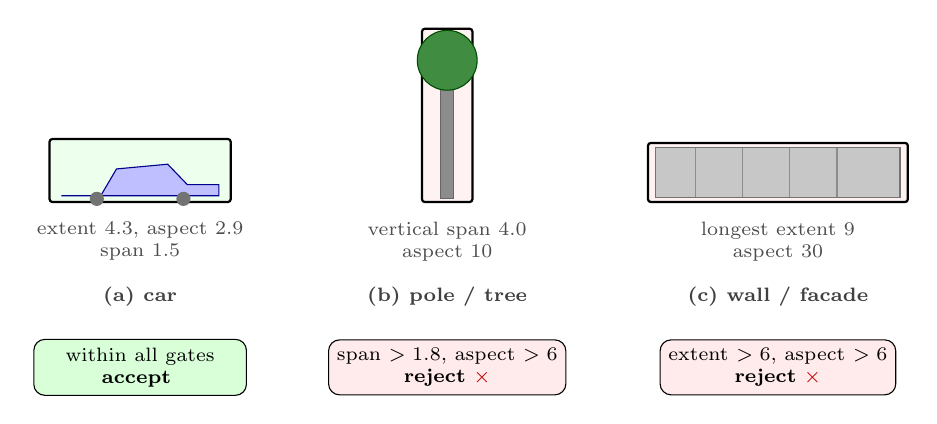
\begin{tikzpicture}[
      font=\footnotesize,
      obb/.style={draw, thick, rounded corners=1pt},
      body/.style={fill=blue!25, draw=blue!55!black},
      verdict/.style={draw, rounded corners, align=center, font=\scriptsize,
        minimum width=27mm, inner sep=3pt},
      dim/.style={font=\scriptsize, align=center, text=black!70},
      plab/.style={font=\scriptsize\bfseries, align=center, text=black!75},
    ]
    %======== (a) car -> accept ========
    \def\ax{0}
    \draw[obb, fill=green!7] (\ax-1.15,1.2) rectangle (\ax+1.15,2.0);
    \fill[body] (\ax-1.0,1.28) -- (\ax-0.5,1.28) -- (\ax-0.3,1.62)
      -- (\ax+0.35,1.68) -- (\ax+0.6,1.42) -- (\ax+1.0,1.42)
      -- (\ax+1.0,1.28) -- cycle;
    \fill[black!55] (\ax-0.55,1.24) circle (0.09);
    \fill[black!55] (\ax+0.55,1.24) circle (0.09);
    \node[dim] at (\ax,0.7) {extent \SI{4.3}{\meter}, aspect \num{2.9}\\span \SI{1.5}{\meter}};
    \node[plab] at (\ax,0.0) {(a) car};
    \node[verdict, fill=green!15] at (\ax,-0.9)
      {within all gates\\\textbf{accept}~\textcolor{green!55!black}{\checkmark}};

    %======== (b) pole / tree -> reject ========
    \def\bx{3.9}
    \draw[obb, fill=red!5] (\bx-0.32,1.2) rectangle (\bx+0.32,3.4);
    \fill[black!45, draw=black!60] (\bx-0.08,1.24) rectangle (\bx+0.08,2.9);
    \fill[green!40!black!75, draw=green!30!black] (\bx,3.0) circle (0.38);
    \node[dim] at (\bx,0.7) {vertical span \SI{4.0}{\meter}\\aspect \num{10}};
    \node[plab] at (\bx,0.0) {(b) pole / tree};
    \node[verdict, fill=red!8] at (\bx,-0.9)
      {span $>\SI{1.8}{\meter}$, aspect $>\num{6}$\\\textbf{reject}~\textcolor{red!75!black}{$\times$}};

    %======== (c) wall / facade -> reject ========
    \def\cx{8.1}
    \draw[obb, fill=red!5] (\cx-1.65,1.2) rectangle (\cx+1.65,1.95);
    \fill[black!22, draw=black!55] (\cx-1.55,1.26) rectangle (\cx+1.55,1.89);
    \foreach \bxx in {-1.05,-0.45,0.15,0.75} {
      \draw[black!45] (\cx+\bxx,1.26) -- (\cx+\bxx,1.89);
    }
    \node[dim] at (\cx,0.7) {longest extent \SI{9}{\meter}\\aspect \num{30}};
    \node[plab] at (\cx,0.0) {(c) wall / facade};
    \node[verdict, fill=red!8] at (\cx,-0.9)
      {extent $>\SI{6}{\meter}$, aspect $>\num{6}$\\\textbf{reject}~\textcolor{red!75!black}{$\times$}};
  \end{tikzpicture}
  \caption[Geometric filtering by OBB gates]{Geometric filtering by oriented-bounding-box
    gates (frozen priors, Table~\ref{tab:pipeline-config}); a cluster survives only within
    every gate. (a)~A car-sized box passes. (b)~A pole or tree fails the vertical-span
    (\SI{1.8}{\meter}) and aspect (\num{6}) gates. (c)~A wall or facade fails the
    longest-extent (\SI{6}{\meter}) and aspect gates.}
  \label{fig:geo-filter}
\end{figure}

\subsection{The Car / Not-Car Point Classifier}
\label{sec:pipeline-classifier}

\noindent \textbf{Input:} car-candidate clusters \quad \textbar \quad \textbf{Output:} per-frame car / not-car label per cluster \vspace{0.5em}

Each surviving cluster is classified as car or not-car by a small
dual branch PointNet. The binary decision
replaces
an earlier multi-class (car/bus/motorcycle) design that was dropped once the data
showed near zero real bus and motorcycle instances, leaving the car-only detector
(Chapter~\ref{ch:introduction}).

\paragraph{Architecture:} The network has two branches
(Figure~\ref{fig:classifier}) and about \num{80000}
parameters, deliberately small:
\begin{itemize}
  \item a point branch that takes \num{512} points (sampled or padded)
    normalised into the unit sphere, and applies shared per point MLPs
    ($3 \to 64 \to 128 \to 256$) followed by a max pool to a \num{256}-d shape
    descriptor;
  \item a bounding box branch that takes an \num{8}-dimensional metric
    feature vector (sorted OBB extents, volume, two aspect ratios,
    $\log(1+\text{point count})$, vertical span), $z$-score normalised, through a
    small MLP to \num{32}-d.
\end{itemize}
The two are concatenated and passed through a small head
($288 \to 128 \to 2$) with dropout. The bounding box branch is what re-injects
absolute metric scale, which the unit sphere normalisation deliberately strips
from the point branch: a distant small car and a nearby one have the same
normalised shape but different real extents, and the metric branch is how the
network sees the difference. There are no T-Nets, since clusters already sit in a
consistent sensor frame.

\begin{figure}[H]
  \centering
  \resizebox{\linewidth}{!}{%
  \begin{tikzpicture}[
      font=\footnotesize, node distance=6mm and 7mm,
      blk/.style={draw, rounded corners, align=center, fill=blue!5, thick,
        minimum height=8mm, inner sep=3pt},
      lrn/.style={blk, fill=orange!12},
      io/.style={draw, ellipse, align=center, fill=black!5, inner sep=2pt},
      arr/.style={-{Stealth[length=2mm]}, thick},
    ]
    \node[io] (cl) at (0,0) {cluster};
    \node[blk] (pts) at (2.3,1.3) {\num{512} points\\unit sphere};
    \node[lrn, right=of pts] (pmlp) {shared MLP\\{\scriptsize $3\!\to\!64\!\to\!128\!\to\!256$}};
    \node[blk, right=of pmlp] (pool) {max-\\pool};
    \node[blk, right=of pool] (pd) {shape\\\num{256}-d};
    \node[blk] (feat) at (2.3,-1.3) {\num{8} OBB\\features};
    \node[lrn, right=of feat] (bmlp) {MLP};
    \node[blk, right=of bmlp] (bd) {metric\\\num{32}-d};
    \node[blk] (cat) at ($(pd.east)+(1.1,-1.3)$) {concat\\\num{288}-d};
    \node[lrn, right=of cat] (head) {head\\{\scriptsize $288\!\to\!128\!\to\!2$}};
    \node[io, right=of head] (out) {car /\\not-car};
    \draw[arr] (cl) |- (pts.west);
    \draw[arr] (cl) |- (feat.west);
    \draw[arr] (pts)--(pmlp); \draw[arr] (pmlp)--(pool); \draw[arr] (pool)--(pd);
    \draw[arr] (feat)--(bmlp); \draw[arr] (bmlp)--(bd);
    \draw[arr] (pd) -| (cat.north);
    \draw[arr] (bd) -| (cat.south);
    \draw[arr] (cat) -- (head);
    \draw[arr] (head) -- (out);
  \end{tikzpicture}%
  }
  \caption[Dual branch classifier]{The dual branch classifier applied to one
    cluster. The point branch takes \num{512} unit sphere normalised points to a
    \num{256}-d shape descriptor; the bounding box branch takes \num{8} metric
    shape features to \num{32}-d. The two are concatenated and passed through a
    small head to a car/not-car decision. Learned blocks are shaded.}
  \label{fig:classifier}
\end{figure}

\paragraph{Training data (mined, not hand labelled):} The classifier is trained
on real LiDAR clusters mined automatically from SemanticKITTI. For each training frame the pipeline's own
stages~1--5 are replayed, the ground truth semantic labels are propagated onto the
surviving clusters by nearest neighbour, and each cluster is labelled car
or not-car by majority vote, keeping only clusters whose majority class
has purity $\geq \num{0.75}$. This yields \num{420333} training clusters
(sequences 00--07, 09, 10) and \num{130394} validation clusters (sequence~08),
with the intrinsic $\approx$21\,\%/79\,\% car/not-car imbalance handled by a
class weighted loss. The key property is that the training clusters are produced
by the same clustering and filtering the classifier meets at inference,
including HDBSCAN splits and filter survivors, so it learns on exactly the
distribution it must classify, at no manual annotation cost.

\paragraph{The from-scratch production classifier:} The final classifier is
trained on the mined real clusters from random initialisation. An earlier
two-stage design first pretrained on synthetic ShapeNet partial renders
(``Stage~A'') and then fine-tuned on the real clusters (``Stage~B''). The
two-stage machinery is reported in Chapter~\ref{ch:evaluation} as an ablation:
a controlled comparison there shows the synthetic pretraining to be redundant given the
mined real clusters, so the final pipeline uses the simpler from scratch checkpoint. The
synthetic pretraining, together with the finding that the sim-to-real gap is total and
symmetric, is presented as a negative result rather than as a contribution.

\paragraph{Training:} The from scratch checkpoint is trained for \num{15} epochs
with Adam (learning rate \num{e-4}, weight decay \num{e-5}) and a step schedule
that halves the rate every \num{10} epochs, at batch size \num{64}. The loss is
cross-entropy weighted by inverse square root class frequency (normalised to unit
mean), which offsets the intrinsic $\approx$21\,\%/79\,\% car/not-car imbalance
without resampling. Training clusters are augmented online with a random rotation
about the vertical axis and Gaussian jitter ($\sigma = \SI{0.005}{\meter}$); the
input is the \num{512}-point cluster of the architecture above. Runs are seeded
and the reported checkpoint is the epoch with the best validation macro-$F_1$; that
value, and the ablation comparison, are reported in Chapter~\ref{ch:evaluation}.

\subsection{Multi-Frame Tracking and Track-Level Filtering}
\label{sec:pipeline-tracker}

\noindent \textbf{Input:} per-frame car detections \quad \textbar \quad \textbf{Output:} tracked cars (oriented boxes $+$ stable track ids) \vspace{0.5em}

Detections are linked across frames by a centroid tracker. Each frame, current detections are matched to existing
tracks by solving a Hungarian assignment on the pairwise centroid distance
matrix; matches beyond \SI{2.0}{\meter} are rejected, unmatched detections start
new tracks, and a track that goes unmatched for more than \num{5} consecutive
frames is retired. This is an offline, centroid only tracker, no motion model,
no appearance, which is adequate here because detection, not association, is
the bottleneck; an IoU-based (SORT-style) tracker is listed as future work.

The tracker also enables a track-level filter that improves precision
(Figure~\ref{fig:tracker}).
Each detection carries the classifier's per frame label; a track is accepted as a
car only if, across its lifetime, it collected at least \num{2} non-rejected
votes, those known votes are a majority of its votes
($\geq \num{0.5}$), and they agree on a single class. A cluster that the
classifier flickers on (a car in one frame, not-car in the next) is thus
resolved by temporal majority rather than trusted per frame. Because this filter
consults the whole track, it is an offline post-processing step, consistent with
the offline scope of the system; its contribution is isolated as an ablation row
in Chapter~\ref{ch:evaluation}. The tracker itself is computationally negligible.

\begin{figure}[H]
  \centering
  \begin{tikzpicture}[
      font=\footnotesize, node distance=6mm and 14mm,
      det/.style={draw, rounded corners, align=center, fill=blue!5, thick,
        minimum height=10mm, minimum width=20mm, inner sep=3pt},
      dec/.style={draw, rounded corners, align=center, fill=orange!10, thick, inner sep=5pt},
      res/.style={draw, ellipse, align=center, inner sep=3pt, minimum width=22mm},
      arr/.style={-{Stealth[length=2mm]}, thick},
      lbl/.style={font=\scriptsize\itshape, text=black!60, align=center},
    ]
    % one track's per-frame detections, linked by centroid association
    \node[det] (d1) {det @ $t$\\[1pt]{\scriptsize\bfseries car}};
    \node[det, right=of d1] (d2) {det @ $t{+}1$\\[1pt]{\scriptsize\bfseries car}};
    \node[det, right=of d2] (d3) {det @ $t{+}2$\\[1pt]{\scriptsize not-car}};
    \draw[arr] (d1)--(d2);
    \draw[arr] (d2)--(d3);
    \node[lbl, above=1mm of d2] {Hungarian assignment, centroid $\le$\,\SI{2}{\meter}};
    \node[lbl, right=6mm of d3, text width=24mm] (ret)
      {unmatched $>\num{5}$ frames\\$\Rightarrow$ track retired};

    % track-level filter over the whole vote sequence
    \node[dec, below=12mm of d2, text width=70mm] (filt)
      {Track-level filter (whole track, offline)\\[2pt]
       $\ge \num{2}$ known votes \;\, $\wedge$ \;\, known vote majority $\ge \num{0.5}$
       \;\, $\wedge$ \;\, single agreed class};
    \draw[arr] (d1) -- (filt.north west);
    \draw[arr] (d2) -- (filt.north);
    \draw[arr] (d3) -- (filt.north east);

    \node[res, fill=green!15, below left=9mm and 3mm of filt] (acc) {accept:\\car track};
    \node[res, fill=black!5, below right=9mm and 3mm of filt] (rej) {reject};
    \draw[arr] (filt.south) -- (acc);
    \draw[arr] (filt.south) -- (rej);
  \end{tikzpicture}
  \caption[Tracker and track-level filter]{The tracker and track-level filter. Per-frame
    detections are linked into tracks by Hungarian assignment on centroid distance (matches
    beyond \SI{2}{\meter} rejected), and the track-level filter resolves each track over its
    whole vote sequence rather than per frame (worked example: votes \{car, car, not-car\}).
    Both steps are offline.}
  \label{fig:tracker}
\end{figure}

\subsection{The Frozen Pipeline Configuration}
\label{sec:pipeline-config}

Table~\ref{tab:pipeline-config} lists the frozen parameter values that produce
every number in this thesis. These parameter values were fixed prior to evaluation and
were not altered to obtain any reported result.

\begin{table}[H]
  \centering
  \caption[Frozen detection pipeline configuration]{Frozen detection pipeline configuration.}
  \label{tab:pipeline-config}
  \begin{tabular}{lll}
    \toprule
    Stage & Parameter & Value \\
    \midrule
    Preprocess & $z$-filter threshold & \SI{-2.0}{\meter} \\
               & voxel size & \SI{0.05}{\meter} \\
               & denoise neighbours / std ratio & \num{20} / \num{2.0} \\
               & voxel before denoise & true \\
    \midrule
    Ground     & RANSAC iterations & \num{300} \\
               & inlier distance & \SI{0.2}{\meter} \\
               & min.\ normal $z$ & \num{0.5} \\
    \midrule
    Clustering & method & HDBSCAN \\
               & min.\ cluster size / min.\ samples & \num{10} / \num{5} \\
               & clustering voxel size & \SI{0.10}{\meter} \\
    \midrule
    Geometric  & min.\ points & \num{15} \\
               & volume range & $[\num{0.5}, \num{50}]\,\si{\meter\cubed}$ \\
               & max.\ longest extent & \SI{6.0}{\meter} \\
               & min.\ top two extents & \SI{0.5}{\meter} / \SI{0.4}{\meter} \\
               & max.\ height above ground & \SI{1.5}{\meter} \\
               & max.\ vertical span & \SI{1.8}{\meter} \\
               & max.\ aspect ratio & \num{6.0} \\
    \midrule
    Classifier & model & dual branch PointNet (binary, from scratch) \\
               & input points & \num{512} \\
    \midrule
    Tracker    & max.\ match distance & \SI{2.0}{\meter} \\
               & max.\ disappeared frames & \num{5} \\
               & min.\ track length & \num{2} \\
               & min.\ known votes / ratio & \num{2} / \num{0.5} \\
    \bottomrule
  \end{tabular}
\end{table}

The completion stage that operates on the tracked car detections
(Figure~\ref{fig:pipeline}, right) is the subject of Section~\ref{ch:completion-method}; the evaluation of
the detections themselves is Chapter~\ref{ch:evaluation}.


%% ===== merged from sec_6_completion_method.tex ===== %%

% Point-Cloud Completion: Method (clean-method-first; false starts gathered in a
% closing "Negative results and lessons" subsection). Folds under Chapter 3.
%
% Scope: this section is the completion METHOD and the debugging narrative that
% produced it. The completion RESULTS (synthetic CD/F, independent-classifier
% plausibility, fidelity) live in Chapter 4 (Evaluation); here we only describe the
% method and defer the full evaluation.
%
% Reframe (2026-09-12): the old self-made completion metric and box-reference
% evaluation are dropped; result numbers migrated to Ch4 per the Ch3=theory rule.
%
% Honesty-phrasing rules applied (personal_agenda P1):
%   - domain-gap failures (#15-19) presented as FINDINGS, not apologies; #26
%     inference bug presented as a debugging lesson.
%   - final path = per-car length estimate ON.
%   - length-prior fallback stated as a live limitation.
%   - measured vs inferred tiers marked; numbers traceable to findings/artifacts.
%
% Figures (all embedded via \graphicspath from the gitignored output/ tree;
% regenerable from the named scripts):
%   Fig 6.1 fig61_partial_compare.py    -> fig61_partials/       (naive vs KITTI-like partial)
%   Fig 6.3 viz_completion.py           -> completion_shape_08.png (final output, output/08)
% Floats set [htbp]. Draft-grade renders; may get a cosmetic restyle in the figure pass.
%
\section{Object Completion}
\label{ch:completion-method}

This part of the method takes each detected car and completes it:
from the one-sided, partial cluster a single LiDAR frame observes, it predicts
the full car surface. The section presents the finished method in the order a
cluster passes through it: the network, its training data, the inference-time
normalisation, the input gate, and the length geometry. The false start that shaped
it, an unsuccessful sim-to-real fine-tuning attempt, is of independent value and is
reported as a negative result in the evaluation (Chapter~\ref{ch:evaluation}) rather
than smoothed over. It is kept out of the method description here, so this section
reads as what the pipeline does rather than how it was arrived at. The engineering
content here is not the network, a standard Point Completion Network (PCN) used off the
shelf, but the data it is trained on and the geometry by which a real partial is
presented to it. The evaluation of the finished method, on synthetic shapes and on real
cars by independent classifier plausibility, is the subject of
Section~\ref{sec:completion-results}; here we describe how the completion is produced.
Figure~\ref{fig:completion-pipeline} gives the full completion path; the subsections
that follow describe each stage in turn.

\begin{figure}[H]
  \centering
  \begin{tikzpicture}[
      font=\small,
      >=Stealth,
      node distance=6mm,
      stage/.style={draw, rounded corners, align=center,
        minimum width=44mm, minimum height=11mm, fill=blue!5, thick},
      learned/.style={stage, fill=orange!12},
      io/.style={draw, ellipse, align=center, fill=black!5,
        minimum width=34mm, minimum height=9mm},
      ms/.style={font=\footnotesize\itshape, text=black!60},
      arr/.style={-{Stealth[length=2.2mm]}, thick},
      grp/.style={draw=black!45, dashed, rounded corners, inner sep=3mm},
      grplab/.style={font=\footnotesize\bfseries, text=black!65},
      legsq/.style={draw, rounded corners, minimum width=5mm, minimum height=3.5mm},
    ]
    \node[io] (in) {Detected car cluster\\{\footnotesize single-frame, partial}};
    \node[stage, below=of in] (gate) {L-shape fit + input gate\\{\footnotesize footprint; reject fragments/merges}};
    \node[stage, below=of gate] (orient) {Reorient to canonical frame\\{\footnotesize gravity $=$ up, L-shape heading $=$ length}};
    \node[stage, below=of orient] (centre) {Full-car centre estimate\\{\footnotesize down-shift $\cdot$ width prior $\cdot$ length}};
    \node[stage, below=of centre] (scale) {Scale-normalise\\{\footnotesize by radius $\div\,\num{1.137}$}};
    \node[learned, below=12mm of scale] (pcn) {PCN completion\\{\footnotesize \num{256}-pt partial $\to$ dense}};
    \node[stage, below=of pcn] (back) {Rotate back to sensor frame};
    \node[io, below=of back] (out) {Completed car\\{\footnotesize dense surface + box}};

    \draw[arr] (in) -- (gate);
    \draw[arr] (gate) -- (orient);
    \draw[arr] (orient) -- (centre);
    \draw[arr] (centre) -- (scale);
    \draw[arr] (scale) -- (pcn);
    \draw[arr] (pcn) -- (back);
    \draw[arr] (back) -- (out);

    \begin{scope}[on background layer]
      \node[grp, fit=(gate)(orient)(centre)(scale)] (prepbox) {};
      \node[grp, fit=(pcn)(back)] (compbox) {};
    \end{scope}
    \node[grplab, rotate=90] at ([xshift=-4mm]prepbox.west) {Canonical-frame prep};
    \node[grplab, rotate=90] at ([xshift=-4mm]compbox.west) {Completion};

    \node[ms, anchor=west] at ([xshift=6mm]prepbox.east|-gate)   {$\to$ oriented footprint};
    \node[ms, anchor=west] at ([xshift=6mm]prepbox.east|-orient) {$\to$ canonical pose};
    \node[ms, anchor=west] at ([xshift=6mm]prepbox.east|-centre) {$\to$ recentred partial};
    \node[ms, anchor=west] at ([xshift=6mm]prepbox.east|-scale)  {$\to$ \num{256}-pt input};
    \node[ms, anchor=west] at ([xshift=6mm]compbox.east|-pcn)    {$\to$ \num{4096}-pt cloud};
    \node[ms, anchor=west] at ([xshift=6mm]compbox.east|-back)   {$\to$ car in sensor frame};

    \node[legsq, fill=blue!5] (lc) at ([yshift=-10mm]out.south west) {};
    \node[right=1.5mm of lc, font=\scriptsize] (lct) {classical (training-free)};
    \node[legsq, fill=orange!12, right=8mm of lct] (ll) {};
    \node[right=1.5mm of ll, font=\scriptsize] {learned};
  \end{tikzpicture}
  \caption[Object completion pipeline]{The object completion pipeline, grouped into two
    phases (dashed): a canonical-frame preparation phase and a completion phase, with each
    stage's output shown at right. The PCN is the only learned stage (shaded); every other
    step is inference-time geometry. Network internals are in Figure~\ref{fig:pcn}.}
  \label{fig:completion-pipeline}
\end{figure}

\subsection{Completion Targets: Single-Frame Car Clusters}
\label{sec:completion-what}

Completion runs on the tracked car detections of Section~\ref{sec:meth-detection}. The input is a
single-frame cluster in the sensor frame, not the accumulated multi-frame
track. This is a deliberate choice with an evidence basis. While temporal accumulation is a common
technique, accumulating a moving car over many frames using a simple centroid tracker
introduces significant motion smear and alignment errors. The slight centroid shifts
frame-to-frame, when accumulated, stretch the car beyond its true boundaries and misalign
the geometric features, producing an invalid completion target that no longer matches the
true car shape. Therefore, a single frame provides one clean, if partial,
observation. Whether completing this partial produces a car-plausible shape on real data
is what Section~\ref{sec:completion-results} measures; this section is how the completion
is produced.

\subsection{The Completion Network (PCN)}
\label{sec:completion-pcn}

We use PCN~\cite{yuan2019pcnpointcompletionnetwork}, an encoder--decoder for point clouds
(Figure~\ref{fig:pcn}). The encoder is a stacked PointNet: shared per point MLPs
lift each point to a local feature, a max pool summarises the whole cloud into a
global vector, that global vector is concatenated back onto every point, and a
second MLP plus max pool stage produces a single \num{1024}-dimensional shape
embedding. The decoder is coarse-to-fine: a fully connected stage predicts
\num{1024} coarse seed points, then a grid folding stage attaches a small
2D grid patch to each seed and learns to fold it into local surface geometry,
densifying the coarse skeleton into the final cloud. Training minimises a
two term Chamfer loss, $\mathrm{CD}_{\text{coarse}} + 0.5\,\mathrm{CD}_{\text{fine}}$;
the fine term is down-weighted so the coarse skeleton is learned first. At
inference the partial is subsampled to \num{256} points before it enters the
encoder.

\begin{figure}[H]
  \centering
  \begin{tikzpicture}[
      font=\footnotesize, node distance=6mm and 7mm,
      blk/.style={draw, rounded corners, align=center, fill=orange!12, thick,
        minimum height=8mm, inner sep=3pt},
      io/.style={draw, ellipse, align=center, fill=black!5, inner sep=2pt},
      arr/.style={-{Stealth[length=2mm]}, thick},
      lbl/.style={font=\footnotesize\itshape, text=black!60},
    ]
    \node[io] (in) {partial\\\num{256} pts};
    \node[blk, right=of in] (ppm) {per point\\MLP};
    \node[blk, right=of ppm] (mp1) {max pool,\\concat back};
    \node[blk, right=of mp1] (mp2) {MLP,\\max pool};
    \node[blk, right=of mp2] (emb) {shape code\\\num{1024}-d};
    \node[blk, below=10mm of emb] (fc) {FC};
    \node[blk, left=of fc] (coarse) {\num{1024}\\coarse seeds};
    \node[blk, left=of coarse] (fold) {grid folding\\{\scriptsize 2D patch / seed}};
    \node[io, left=of fold] (out) {dense car\\\num{4096} pts};
    \draw[arr] (in)--(ppm); \draw[arr] (ppm)--(mp1); \draw[arr] (mp1)--(mp2);
    \draw[arr] (mp2)--(emb); \draw[arr] (emb)--(fc); \draw[arr] (fc)--(coarse);
    \draw[arr] (coarse)--(fold); \draw[arr] (fold)--(out);
    \node[lbl, above=1mm of mp1] {encoder (stacked PointNet)};
    \node[lbl, below=1mm of coarse] {decoder (coarse-to-fine)};
  \end{tikzpicture}
  \caption[Completion network (PCN)]{The completion network (PCN). A stacked PointNet
    encoder maps the \num{256}-point partial to a \num{1024}-d global shape code;
    a coarse-to-fine decoder predicts \num{1024} seed points and folds a small 2D
    grid patch onto each to produce the dense \num{4096}-point car. Every block is
    learned; the architecture is used off the shelf and unmodified.}
  \label{fig:pcn}
\end{figure}

The architecture is not a contribution and was not modified; the controlled comparison
against PoinTr that justifies keeping PCN, a small synthetic edge and equivalent
real data behaviour, is reported with the completion ablations
(Section~\ref{sec:abl-completion}). What makes PCN
work on real cars is not the weights but the two subsections that follow: the
distribution of partials it is trained on, and the frame a real partial is normalised
into at inference.

\subsection{Training Data: KITTI-Like Partials}
\label{sec:completion-kittilike}

PCN is trained on synthetic partials, and those partials must match the distribution
of the real clusters it meets at inference or the network sees a different input at
test time than it was trained on. A derisk study comparing candidate partial
generators against real seq-08 clusters isolated three properties a naive
generator gets wrong: it sampled a dense pinhole depth render, skipped the
\SI{0.05}{\meter} voxelisation and ground removal the real input has been through, and
added range proportional noise (up to \SI{0.15}{\meter} at \SI{30}{\meter}) that
washed out the scan ring banding real Velodyne data shows.

The generator used makes the synthetic partial match the real one: it orients the
ShapeNet car to gravity, casts a single HDL-64E viewpoint (64 elevation beams,
\SI{0.09}{\degree} horizontal resolution) from a sensor at \SI{1.73}{\meter} and
a sampled range of \SIrange{8}{30}{\meter}, adds small absolute noise
(\SI{0.015}{\meter}), voxelises at \SI{0.05}{\meter} to match the pipeline, and
removes points within \SI{0.30}{\meter} of the ground plane. The dense complete
mesh sample remains the target. The PCN model retrained on these partials
is in-distribution with the real input, and on a held-out
synthetic set produces clean cars rather than blobs; its synthetic Chamfer and F-score are
reported in Chapter~\ref{ch:evaluation}. Figure~\ref{fig:kitti-like-partial} contrasts the
naive and KITTI-like partials for the same ShapeNet car.

\paragraph{Training:} PCN is trained on the KITTI-like synthetic partials (input
\num{256} points, target the dense mesh sample) for \num{100} epochs with Adam
(learning rate \num{e-4}, weight decay \num{e-6}) and a step schedule that halves
the rate every \num{40} epochs, at batch size \num{8}, minimising the two term
Chamfer loss above. No real cars enter training; the reported model
is the best validation loss epoch. The subsequent geometry
work is all inference time and does not retrain the network.

\begin{figure}[htbp]
  \centering
  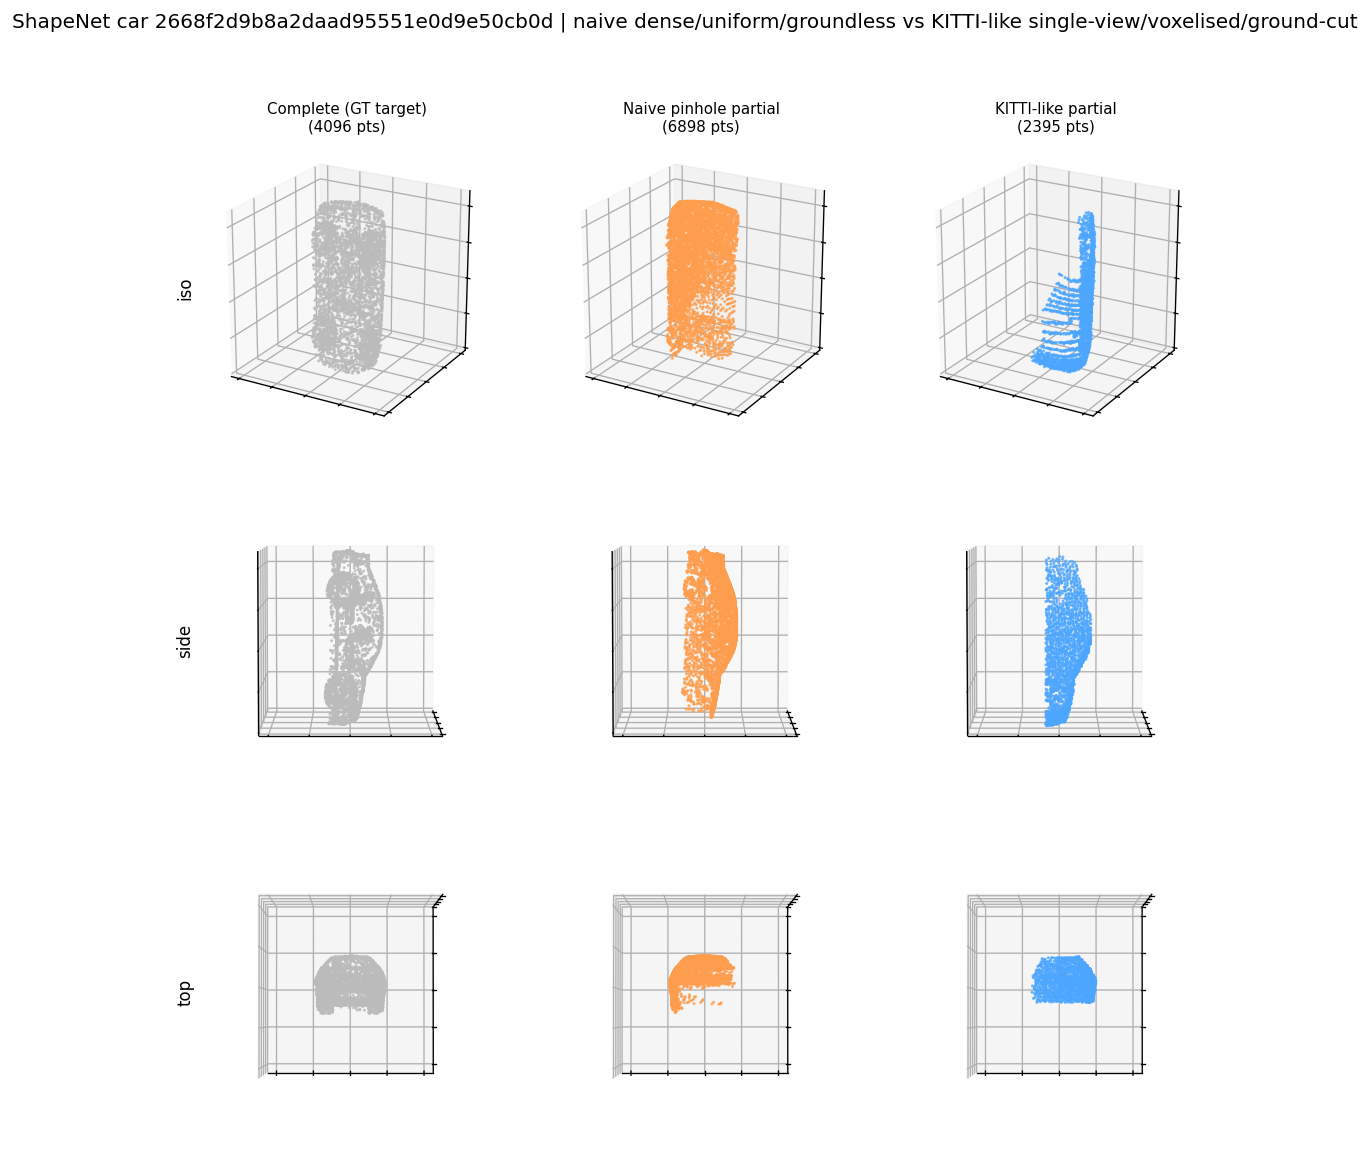
\includegraphics[width=\linewidth]{fig61_partials/partials_2668f2d9b8a2daad95551e0d9e50cb0d.png}
  \caption[Training input distribution]{The training input distribution: one ShapeNet car
    with its complete surface target (left, grey) and two candidate training inputs, the naive
    pinhole partial (centre, orange) and the KITTI-like partial (right, blue) that reproduces
    real LiDAR (scan-ring banding, single-viewpoint coverage, \SI{0.05}{\meter} voxelisation,
    ground cut). These are training inputs, not completion outputs.}
  \label{fig:kitti-like-partial}
\end{figure}

\subsection{Inference-Time Partial Normalisation}
\label{sec:completion-normalisation}

\noindent \textbf{Input:} gated car cluster (sensor frame) $+$ L-shape heading and per-car length \quad \textbar \quad \textbf{Output:} \num{256}-point partial in the canonical car frame (centred, scale-normalised) \vspace{0.5em}

PCN is trained on shapes expressed in a fixed canonical car frame, centred on the
true car centre and scaled by the true car radius. At inference a real partial
must therefore be mapped into that same frame before it is completed; anything else
hands the network a normalisation it never saw during training. Reconstructing that
frame from a one-sided partial is non-trivial, because a partial reveals neither the
true centre nor the true radius directly. The inference geometry
reconstructs it in three steps:

\begin{itemize}
  \item Reorientation. The sensor frame is rotated into the canonical
    car frame (X${}={}$width, Y${}={}$up, Z${}={}$length): gravity maps to the
    up axis, and the horizontal heading axis maps to length. Heading comes from the
    L-shape footprint fit (Section~\ref{sec:completion-lshape}), not a principal axis
    alignment.
  \item Full car centre estimate. A one-sided partial's bounding box
    centre is not the car centre, so the centre is corrected on each axis: shift
    down to undo the upward bias from the ground cut (the dominant
    correction, \SI{0.25}{\meter}); push outward along width toward the
    occluded far side using a full-car width prior (\SI{1.9}{\meter}); and push
    along length toward the occluded far end (Section~\ref{sec:completion-length}).
  \item Scale. Normalise by the maximum point-to-centre distance divided
    by a fixed scale correction (\num{1.137}), the calibrated ratio between a
    one-sided partial radius and the true car radius.
\end{itemize}

With this path the same real seq-08 clusters recover the correct pose and scale; the
ablation isolating this normalisation against a naive partial frame alternative, and the
box overlap gains it produces, is reported with the completion ablations
(Section~\ref{sec:abl-completion}). Viewed in the
canonical car frame, the corrected completions are recognisably car-shaped: they
recover the car footprint in bird's-eye view and a rough side silhouette
(roofline included) even from very sparse input, a clean car footprint from a
\num{64}-point cluster in the extreme case. We are nonetheless careful about the
strength of the claim: crispness varies with input density (cleaner on
well-observed cars, blobbier on the sparsest), and a completion is a filled
\num{4096}-point cloud rather than a CAD clean surface. The sharpest completions
are the in-distribution synthetic ones of
Section~\ref{sec:completion-kittilike}; on real data the normalisation's value is
corrected geometry, pose and scale, and the car plausibility of the completed shape
that Section~\ref{sec:completion-results} reports. A calibration study on synthetic cars
further identified the residual dominant error as centre estimation, not scale,
which is what motivates the geometry work in the rest of this section.

\subsection{L-Shape Gating of Completion Inputs}
\label{sec:completion-lshape}

\noindent \textbf{Input:} detected car cluster (single-frame partial) \quad \textbar \quad \textbf{Output:} fitted footprint $+$ accept/reject decision (fragments and merges rejected) \vspace{0.5em}

Even with correct normalisation, some clusters cannot complete into a plausible
car because the input is not one car: HDBSCAN fragments (part of a car) and
merges (two cars, or a \SI{90}{\degree} heading error) both feed the completion
network implausible input. To detect them we fit the cluster's ground plane footprint with a
search-based L-shape fit~\cite{zhang2017lshape}, which scores edge adherence over
candidate yaw angles and stays well-defined on near square footprints where PCA
degenerates. The fitted footprint gives an input quality gate: a
cluster is rejected as a fragment if its fitted length is below \SI{2.7}{\meter},
or as a merge if its fitted width exceeds \SI{2.3}{\meter}
(Figure~\ref{fig:lshape-gate}), so the gate keeps implausible inputs out of the completion
network rather than relying on it to fix them.

On seq-08 every implausible completion
originated from a fragment or merge input, so the gate's effect on completion quality
is a clean ablation, reported in Section~\ref{sec:abl-completion}. An honest secondary
finding from the same study: the L-shape heading itself is neutral against plain PCA on
real data, the fit earns its place by detecting bad inputs, not by giving a
better heading.

\begin{figure}[H]
  \centering
  \begin{tikzpicture}[
      font=\footnotesize, scale=0.6,
      pt/.style={circle, fill=blue!70!black, inner sep=0pt, minimum size=2.4pt},
      fitobb/.style={draw=black!70, thick, densely dashed},
      ledge/.style={draw=orange!80!black, line width=0.8pt},
      dimarr/.style={<->, >=Stealth, black!60},
      dlab/.style={font=\scriptsize, text=black!80, align=center},
      verdict/.style={draw, rounded corners, align=center, font=\scriptsize, inner sep=3pt},
      plab/.style={font=\scriptsize\bfseries, align=center, text=black!75},
    ]
    %======== (a) single car -> accept ========
    \def\ao{0}
    \draw[fitobb] (\ao,0) rectangle (\ao+4.3,1.8);
    \draw[ledge] (\ao,1.8) -- (\ao,0) -- (\ao+4.3,0);
    \foreach \x in {0,0.3,...,4.3}{ \node[pt] at (\ao+\x,0){}; }
    \foreach \y in {0,0.3,...,1.8}{ \node[pt] at (\ao,\y){}; }
    \draw[dimarr] (\ao,-0.45) -- (\ao+4.3,-0.45);
    \node[dlab] at (\ao+2.15,-0.95) {$L=\SI{4.3}{\meter}\ge\SI{2.7}{\meter}$};
    \draw[dimarr] (\ao-0.45,0) -- (\ao-0.45,1.8);
    \node[dlab, rotate=90] at (\ao-0.95,0.9) {$W=\SI{1.8}{\meter}\le\SI{2.3}{\meter}$};
    \node[plab] at (\ao+2.15,-1.7) {(a) single car};
    \node[verdict, fill=green!15] at (\ao+2.15,-2.7) {\textbf{accept}~\textcolor{green!55!black}{\checkmark}};

    %======== (b) fragment -> reject ========
    \def\bo{7.4}
    \draw[fitobb] (\bo,0) rectangle (\bo+2.0,1.3);
    \draw[ledge] (\bo,1.3) -- (\bo,0) -- (\bo+2.0,0);
    \foreach \x in {0,0.3,...,2.0}{ \node[pt] at (\bo+\x,0){}; }
    \foreach \y in {0,0.3,...,1.3}{ \node[pt] at (\bo,\y){}; }
    \draw[dimarr] (\bo,-0.45) -- (\bo+2.0,-0.45);
    \node[dlab] at (\bo+1.0,-0.95) {$L=\SI{2.0}{\meter}<\SI{2.7}{\meter}$};
    \node[plab] at (\bo+1.0,-1.7) {(b) fragment};
    \node[verdict, fill=red!8] at (\bo+1.0,-2.7) {\textbf{reject:} fragment~\textcolor{red!75!black}{$\times$}};

    %======== (c) merge (two cars) -> reject ========
    \def\co{12.0}
    \draw[fitobb] (\co,0) rectangle (\co+4.6,3.2);
    \draw[black!35] (\co+0.2,0.2) rectangle (\co+4.4,1.5);
    \draw[black!35] (\co+0.2,1.7) rectangle (\co+4.4,3.0);
    \draw[ledge] (\co,3.2) -- (\co,0) -- (\co+4.6,0);
    \foreach \x in {0,0.3,...,4.6}{ \node[pt] at (\co+\x,0){}; }
    \foreach \y in {0,0.3,...,3.2}{ \node[pt] at (\co,\y){}; }
    \foreach \x in {0,0.3,...,4.6}{ \node[pt] at (\co+\x,3.2){}; }
    \draw[dimarr] (\co-0.45,0) -- (\co-0.45,3.2);
    \node[dlab, rotate=90] at (\co-0.95,1.6) {$W=\SI{3.2}{\meter}>\SI{2.3}{\meter}$};
    \node[plab] at (\co+2.3,-1.7) {(c) merge (two cars)};
    \node[verdict, fill=red!8] at (\co+2.3,-2.7) {\textbf{reject:} merge~\textcolor{red!75!black}{$\times$}};
  \end{tikzpicture}
  \caption[L-shape gating of completion inputs]{L-shape gating of completion inputs. Each
    cluster's ground-plane footprint (blue points) is fit with a search-based L-shape (orange
    edges), and the fitted rectangle (dashed) yields a length and a width. (a)~A single car
    clears both gates ($L\ge\SI{2.7}{\meter}$, $W\le\SI{2.3}{\meter}$). (b)~A fragment is too
    short ($L<\SI{2.7}{\meter}$). (c)~A merge is over-wide ($W>\SI{2.3}{\meter}$).}
  \label{fig:lshape-gate}
\end{figure}

\subsection{Per-Car Length Estimation}
\label{sec:completion-length}

\noindent \textbf{Input:} the track's gate-passed footprint length fits \quad \textbar \quad \textbf{Output:} per-car length estimate (feeds the centre estimate) \vspace{0.5em}

The canonical frame centre estimate re-centres the occluded lateral side and the
ground cut, but a partial truncated at the occluded far end is normalised
around its observed near portion, so PCN's output tends to stop short of the far end,
the least covered region of a one-sided car. Two successive fixes address it, both
inference only (no retraining).

\paragraph{The fixed length prior:} A longitudinal, extend only
push mirrors the width prior along the length axis: the centre is pushed toward
the occluded far end so the completion reaches an assumed full car length of
\SI{4.14}{\meter}, a population median car length. A larger \SI{4.5}{\meter} prior
was rejected because it over-extended genuinely compact cars.

\paragraph{The per-car estimate:} A single \SI{4.14}{\meter}
prior is a population median, so it is wrong in both tails, it over-extends
compact cars and under-extends long ones. It is replaced by a per-car length estimate:
the \nth{90} percentile of the car's own
gate passed footprint length fits, plus a \SI{0.12}{\meter} bias correction,
falling back to the fixed prior when a track has fewer than \num{5} gate passed
frames. The aggregate is a quantile, not the maximum, because a single
contaminated L-shape fit would set the maximum. This is a per track quantity, so the
pipeline (which owns the track) computes it and passes it in; the completion module itself
stays stateless.

\paragraph{Limitation:} The fallback is not rare: a non-trivial fraction of tracks have
fewer than five gate passed frames and fall back to the fixed prior. This is stated as a
live limitation, not a solved problem; the exact fallback rate on sequence~08 is reported
with the completion results, and it is revisited in the discussion.

\subsection{The End-to-End Completion Path}
\label{sec:completion-summary}

\noindent \textbf{Input:} single-frame car cluster (sensor frame) \quad \textbar \quad \textbf{Output:} completed dense car (\num{4096}-point surface $+$ box, sensor frame) \vspace{0.5em}

To summarise, a single-frame car cluster is completed by: fitting its footprint
and rejecting fragments and merges (L-shape gate); reorienting it into the
canonical car frame with no PCA; estimating the full car centre (down-shift for
the ground cut, width prior for the occluded side, per-car length estimate for
the occluded far end); normalising by the scale corrected radius; running the
KITTI-like-trained PCN; and rotating the output back to the sensor frame. The frozen
geometric priors used across these inference steps are collected in
Table~\ref{tab:completion-config}. Every
step is inference-time geometry except the one-off retraining on KITTI-like
partials; no step fine-tunes on the evaluation cars.

Figure~\ref{fig:completion-shape} shows what this path produces on real seq-08
cars across the input density range, in the canonical car frame. The completed
cloud (green) fills the car footprint and a rough side silhouette that the
single-frame partial (blue) leaves one-sided, recognisably car-shaped down to a
\num{64}-point input. Consistent with the caveats above, the sparsest inputs complete
more coarsely and can inflate the width, and the clouds are filled rather than CAD clean.
The point here is qualitative shape; the quantitative real data assessment,
whether the completed cloud reads as a car to an independent classifier, is what
Section~\ref{sec:completion-results} sets out to measure.

\begin{figure}[htbp]
  \centering
  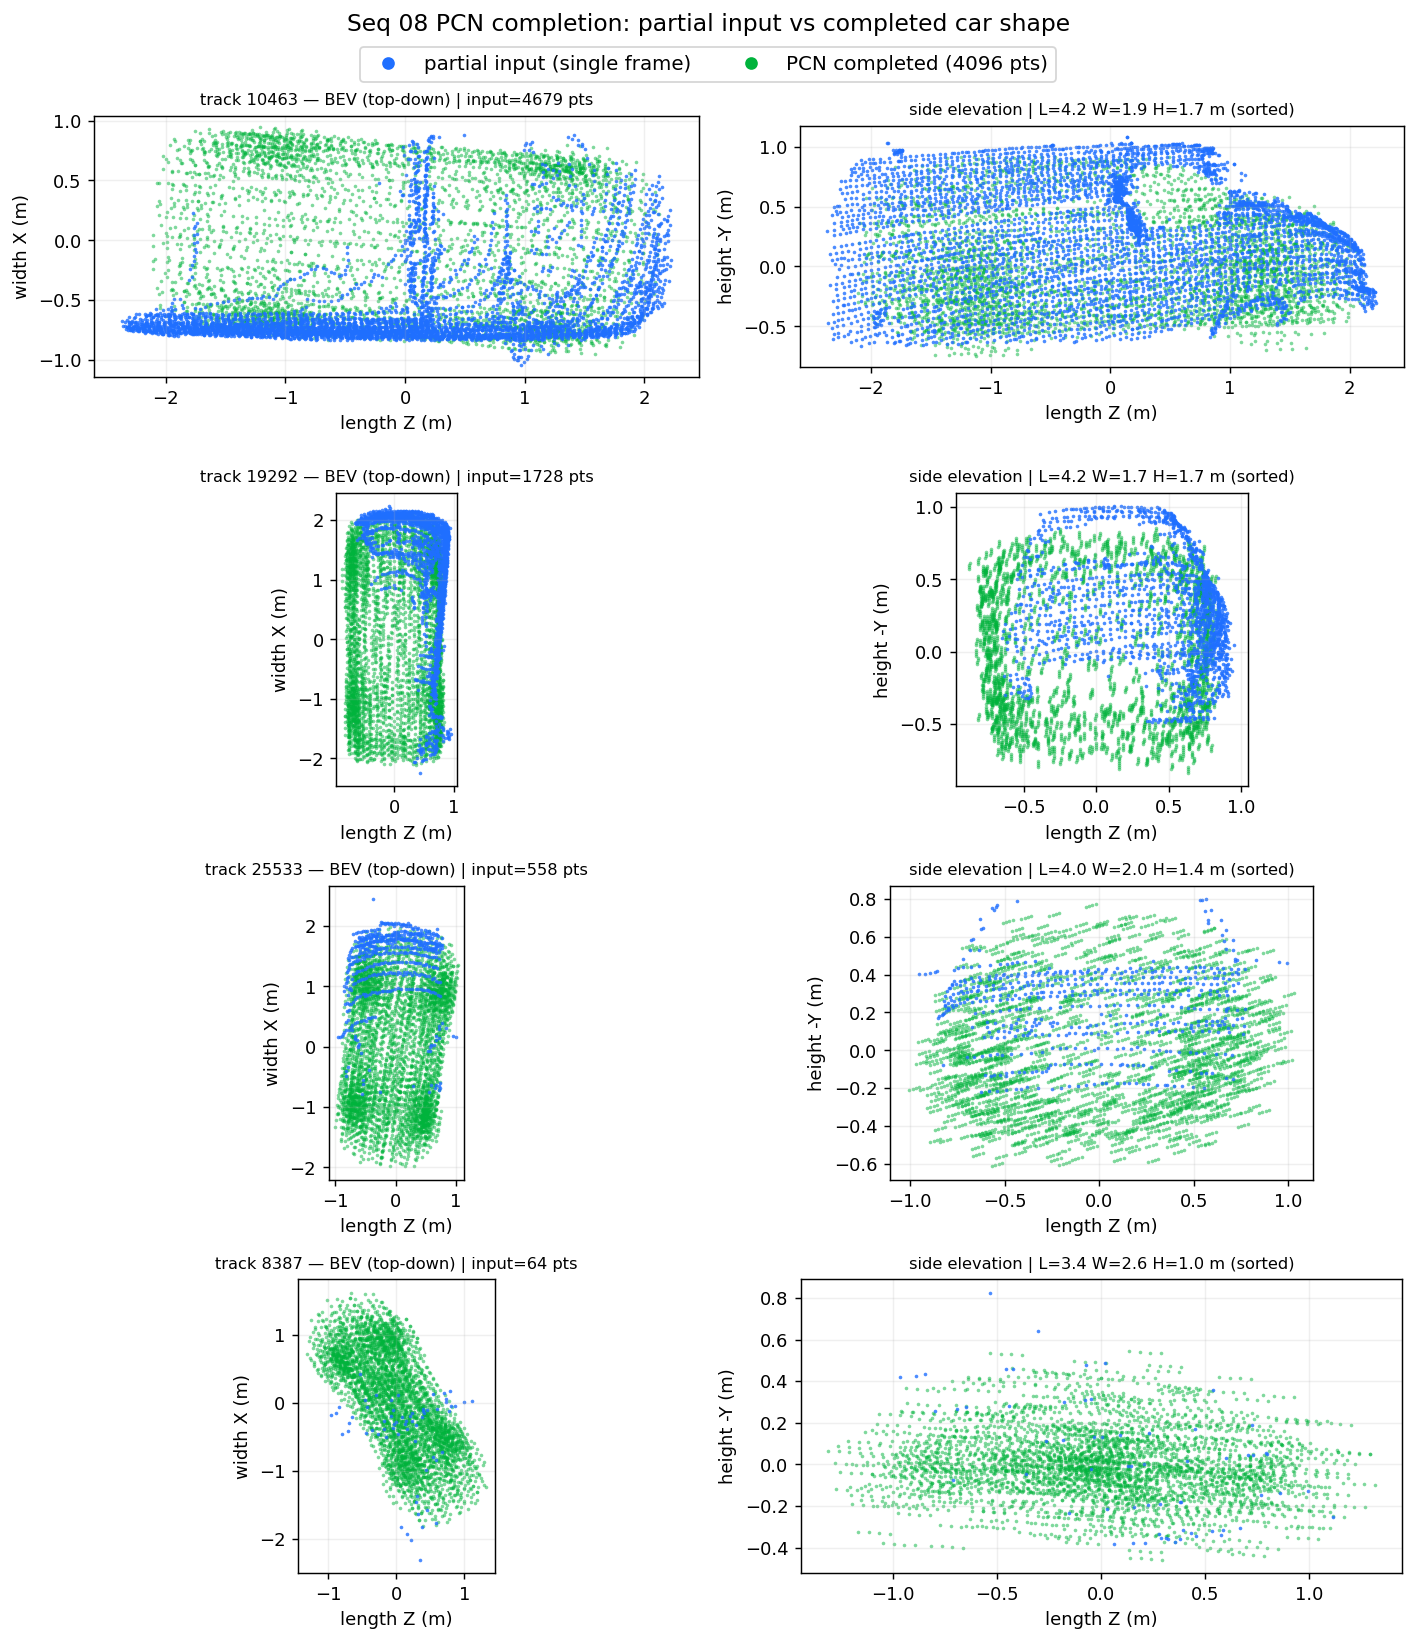
\includegraphics[width=\linewidth]{completion_shape_08.png}
  \caption[Completions on real cars]{The final completion path on real cars,
    four tracks spanning the input density range, each in the canonical car frame: bird's-eye
    view (left of each pair) and side elevation (right). Blue is the single-frame partial
    input, green the PCN completion.}
  \label{fig:completion-shape}
\end{figure}

\begin{table}[H]
  \centering
  \caption[Frozen completion pipeline configuration]{Frozen completion pipeline
    configuration. These geometric priors are fixed at inference for all evaluated cars.}
  \label{tab:completion-config}
  \begin{tabular}{lll}
    \toprule
    Stage & Parameter & Value \\
    \midrule
    L-Shape Gating & min.\ fitted length (fragment) & \SI{2.7}{\meter} \\
                   & max.\ fitted width (merge) & \SI{2.3}{\meter} \\
    \midrule
    Normalisation  & ground cut down-shift & \SI{0.25}{\meter} \\
                   & full-car width prior & \SI{1.9}{\meter} \\
                   & radius scale correction & \num{1.137} \\
    \midrule
    Length Geometry & fixed length prior & \SI{4.14}{\meter} \\
                    & min.\ gate-passed frames & \num{5} \\
                    & length bias correction & \SI{0.12}{\meter} \\
    \bottomrule
  \end{tabular}
\end{table}

\section{Summary and Methodological Limitations}
\label{sec:meth-limitations}

This chapter has set out the full method: the modular detection pipeline that turns a
raw scan into car detections, and the single-frame completion path with its input gate and
length prior. Several limitations are built into these choices and are flagged here so the
evaluation is read with them in view; each is taken up in full in the discussion of
Chapter~\ref{ch:conclusion}.

\begin{itemize}
  \item Ground model: a single global RANSAC plane assumes near planar
    ground; it holds on the flat urban sequences used here but would degrade on
    strong slopes, where a grid-based model (future work) would be needed
    (Section~\ref{sec:pipeline-ground}).
  \item Offline by design: the tracker and track-level filter consult the
    whole sequence, and the pipeline runs far below sensor rate; real-time operation is
    out of scope (Section~\ref{sec:pipeline-overview}).
  \item Single-frame, static car completion: completion runs on one frame's
    cluster; moving cars are completed but are considered separately, and no completion is
    scored against an accumulated multi-frame shape (Section~\ref{sec:completion-what}).
  \item Length prior fallback: the per-car length estimate falls back to the
    fixed \SI{4.14}{\meter} prior on tracks with fewer than five gate passed frames, and a
    residual far end under-extension on long cars is a characterised, not eliminated, limit
    (Section~\ref{sec:completion-length}).
  \item Synthetic only completion training: PCN sees only synthetic
    KITTI-like partials; real data fine-tuning was a negative result, so a sim-to-real
    residual remains (Chapter~\ref{ch:evaluation}).
\end{itemize}

With these caveats stated, Chapter~\ref{ch:evaluation} puts each component to the test:
the detection operating point and its ablations, the recall root cause, and the
completion results (synthetic fidelity and independent classifier plausibility).
Chapter~\ref{ch:conclusion} then returns to the limitations above, alongside the evaluation
questions the results raise.

